\documentclass[conference]{IEEEtran}
\IEEEoverridecommandlockouts
\usepackage{cite}
\usepackage{amsmath,amssymb,amsfonts}
\usepackage{algorithmic}
\usepackage{graphicx}
\usepackage{textcomp}
\usepackage{xcolor}
\usepackage{booktabs}
\usepackage{float}
\usepackage{multirow}
\usepackage{url}
\usepackage{hyperref}

% ---- Conference Formatting Overrides ----
% Font: Times New Roman
\usepackage{mathptmx}
\usepackage[T1]{fontenc}

% Line spacing: 1.5
\usepackage{setspace}
\onehalfspacing

% Font sizes: Title 16pt, Sub-title 14pt, Body 12pt
\usepackage{titlesec}
\renewcommand{\normalsize}{\fontsize{12}{18}\selectfont}
\renewcommand{\small}{\fontsize{10}{14}\selectfont}
\renewcommand{\footnotesize}{\fontsize{9}{12}\selectfont}
\renewcommand{\scriptsize}{\fontsize{8}{10}\selectfont}
\renewcommand{\large}{\fontsize{14}{17}\selectfont}
\renewcommand{\Large}{\fontsize{14}{17}\selectfont}
\renewcommand{\LARGE}{\fontsize{16}{20}\selectfont}

% Section headings: 14pt bold
\titleformat{\section}{\fontsize{14}{17}\selectfont\bfseries\centering}{\thesection.}{0.5em}{}
\titleformat{\subsection}{\fontsize{14}{17}\selectfont\bfseries}{\thesubsection.}{0.5em}{}
\titlespacing{\section}{0pt}{12pt}{6pt}
\titlespacing{\subsection}{0pt}{10pt}{4pt}

\def\BibTeX{{\rm B\kern-.05em{\sc i\kern-.025em b}\kern-.08em
    T\kern-.1667em\lower.7ex\hbox{E}\kern-.125emX}}
\begin{document}

\title{\fontsize{16}{20}\selectfont Weather-Based Solar Energy Prediction Using Random Forest Regression and Planning System Using Generative AI}

\author{
\IEEEauthorblockN{1\textsuperscript{st} Al Ameen H}
\IEEEauthorblockA{\textit{Dept. of Information Technology} \\
\textit{Dhanalakshmi Srinivasan College}\\
\textit{of Engineering and Technology}\\
Mamallapuram, Chennai, Tamil Nadu \\
alameenofficial11@gmail.com}
\and
\IEEEauthorblockN{2\textsuperscript{nd} Hemachandiran J}
\IEEEauthorblockA{\textit{Dept. of Information Technology} \\
\textit{Dhanalakshmi Srinivasan College}\\
\textit{of Engineering and Technology}\\
Mamallapuram, Chennai, Tamil Nadu \\
hemachandiranj.it2022@dscet.ac.in}
\and
\IEEEauthorblockN{3\textsuperscript{rd} Ranjitha}
\IEEEauthorblockA{\textit{Asst. Professor, Dept. of IT} \\
\textit{Dhanalakshmi Srinivasan College}\\
\textit{of Engineering and Technology}\\
Mamallapuram, Chennai, Tamil Nadu \\
ranjitha.it@dscet.ac.in}
\and
\IEEEauthorblockN{4\textsuperscript{th} Ravi Kumar}
\IEEEauthorblockA{\textit{HOD, Dept. of IT} \\
\textit{Dhanalakshmi Srinivasan College}\\
\textit{of Engineering and Technology}\\
Mamallapuram, Chennai, Tamil Nadu \\
ravikumar.ithod@dscet.ac.in}
}

\maketitle

\begin{abstract}
As rooftop solar photovoltaic (PV) installations become increasingly popular across India, there is a growing need for reliable energy forecasting tools to help homeowners make confident, informed financial decisions. In this paper, we introduce SolarPredict: a full-stack, web-based decision support system. It combines machine learning-based solar energy predictions with real-time weather data, detailed financial modeling, and an advisory layer powered by Generative AI. At its core, the prediction engine relies on a Random Forest Regressor. We trained it using 136,476 operational records from two active solar power plants, and it achieved an impressive 0.853 coefficient of determination (R\textsuperscript{2}) alongside a 0.032 normalized mean absolute error (MAE) on unseen test data. Alongside the predictive features, we integrated Google Gemini to act as an intelligent planning assistant. It translates raw technical outputs into personalized, easy-to-read advice on everything from financial returns to optimal times for running household appliances. The underlying architecture relies on a three-tier microservice model---specifically a React frontend, an Express.js API gateway, and a FastAPI machine learning inference service connected to a MongoDB database. Moreover, SolarPredict pulls live weather conditions via the OpenWeather API and directly incorporates up-to-date Indian government subsidies, like those under the PM Surya Ghar scheme. Ultimately, our system goes beyond simply estimating solar outputs; it actively guides homeowners through the financial and practical realities of adopting solar energy.
\end{abstract}

\begin{IEEEkeywords}
solar energy prediction, random forest regression, generative AI, decision support system, machine learning, photovoltaic, weather-based forecasting, renewable energy, smart planning
\end{IEEEkeywords}

\section{Introduction}

India has set a major goal for itself: reaching 500~GW of renewable energy capacity by 2030, which is a key piece of its commitment to the Paris Agreement \cite{b1}. Rooftop solar photovoltaic (PV) setups offer a fantastic way to push decentralized energy generation, especially in everyday residential neighborhoods. Recognizing this, the Indian government launched the PM Surya Ghar: Muft Bijli Yojana scheme in 2024. This initiative offers subsidies up to INR~78,000 to help solarize roughly ten million households \cite{b2}. However, even with these strong financial incentives, typical homeowners struggle to accurately figure out how much energy they can realistically produce, calculate their financial returns, or understand how local weather shifts will eventually affect their panels.

To be fair, predicting solar energy generation is naturally difficult because it relies heavily on shifting atmospheric elements like sunlight levels, ambient temperature, cloud cover, humidity, and wind speed \cite{b3}. Traditional physics-based clear-sky models offer a good starting theory, but they often struggle to account for the chaotic reality of actual weather patterns. On the other hand, machine learning techniques---especially ensemble methods like Random Forests---have proven highly effective at mapping the complicated, nonlinear connections between the weather and power output \cite{b4}.

Beyond just doing the math, the recent boom in Generative AI and Large Language Models (LLMs) provides a massive opportunity. We can now build intelligent planning assistants that translate complicated technical forecasts into plain, helpful language \cite{b11}. Combining AI-driven language tools with machine learning means we can go structurally further than predicting output: we can offer personalized advice on panel installation, cost savings, and day-to-day energy management.

When looking at the current tools available in the literature, they typically hyper-focus on either boosting prediction accuracy or linking basic system components together. Most fail to offer a unified pipeline that successfully moves a user from fetching local weather data through energy generation modeling all the way to plain-English financial advice. What's more, most existing software is built strictly for large utility companies, missing the mark entirely when it comes to the clean, intuitive interfaces that regular residential consumers actually want to use \cite{b5}.

In this paper, we aim to bridge that exact gap with SolarPredict---a comprehensive, web-based prediction and planning system. Specifically, our work offers the following main contributions:

\begin{itemize}
\item We developed a Random Forest Regressor trained directly on real-world solar plant data \cite{b12}. The model utilizes nine specifically engineered features, including cyclical time representations and synthetic weather data, to keep energy predictions highly accurate.
\item We actively pull down live weather metrics through the OpenWeather API, giving every user localized and up-to-date forecasts.
\item The system provides a thorough financial breakdown, projecting total installation costs, PM Surya Ghar subsidy application, Return on Investment (ROI), and a detailed 25-year estimate of net savings.
\item We built an interactive planner driven by Google Gemini. This Generative AI component offers custom solar advice, generates automated summaries, fields natural language questions, and proposes smart appliance schedules.
\item We deployed the entire service using a modern microservice approach equipped with JWT-authenticated user profiles, allowing individuals to track their historic predictions and watch system performance over time.
\end{itemize}

The rest of the paper follows this flow: Section~II takes a look at existing work in solar prediction and AI planning tools. Section~III breaks down how our system is architected. Section~IV details the machine learning model's inner workings. Section~V dives into our Generative AI planner and its decision-support capabilities. In Section~VI, we outline our experimental results. Finally, Section~VII wraps up our findings and discusses where this research could potentially head next.

\section{Related Work}

\subsection{Solar Energy Prediction Methods}

Historically, efforts to predict solar energy have fallen into three main buckets: physical models, statistical models, and machine learning models \cite{b3}, \cite{b14}, \cite{b16}. Physical models, like the classic Hottel clear-sky model, calculate solar irradiance by crunching numbers related to atmospheric transmittance, solar geometry, and geography. While they look great on paper, they often fall short when dealing with unpredictable cloud cover and specific local weather quirks \cite{b6}.

On the statistical side, time-series techniques like Autoregressive Integrated Moving Average (ARIMA) and exponential smoothing have seen quite a bit of use \cite{b15}. The drawback here is that they tend to assume linear relationships. Unfortunately, the interactions between weather conditions and power generation are incredibly nonlinear, making these models a bit too rigid for real-world application \cite{b7}, \cite{b18}.

Because of these limitations, machine learning methods have strongly stepped into the spotlight. They excel at learning complex, nonlinear rules straight from the data. Researchers have rigorously tested tools like Support Vector Regression (SVR), Artificial Neural Networks (ANN), and ensemble techniques like Random Forest and Gradient Boosting \cite{b4}, \cite{b19}. Deep learning---specifically Long Short-Term Memory (LSTM) networks---has also shown great promise for mapping out solar power over time \cite{b13}, \cite{b17}. Out of all these options, Random Forest stands out. It consistently performs well across messy datasets, fights off overfitting naturally, handles mixed data types easily, and makes it easy for us to understand which features are actually driving the predictions \cite{b8}.

\subsection{Decision Support Systems for Solar Energy}

There is no shortage of web-based tools out there for predicting solar potential. Google's Project Sunroof does a great job using aerial imagery and 3D modeling to gauge rooftop capacity \cite{b9}. Similarly, the National Renewable Energy Laboratory (NREL) offers the PVWatts Calculator, leaning on physics-based estimations for PV output \cite{b10}. The core issue? These tools are heavily geared towards the US market. They completely lack the financial frameworks necessary to account for Indian subsidy schemes and local electricity pricing. Given recent studies underscoring the massive potential for rooftop solar across Indian states, it's clear that a localized, India-specific decision platform is long overdue \cite{b20}.

\subsection{Generative AI in Energy Systems}

Lately, Generative AI has cracked open entirely new possibilities for managing energy systems. Researchers have started using Large Language Models to chat with energy data, automate reporting, and make AI forecasting significantly easier to digest \cite{b11}. That said, dropping Gen AI into a solar prediction system as a dedicated planning and advisory layer hasn't been done much at all. We are extending this fresh avenue of research by tying the analytical heavy-lifting of a Random Forest predictor to a user-friendly Gemini LLM interface. This essentially bridges the gap between raw quantitative predictions and qualitative, personalized advice for Indian consumers.

\section{System Architecture and Design}

\subsection{Overall Architecture}

SolarPredict follows a three-tier microservice architecture as illustrated in Fig.~\ref{fig:arch}. The system comprises three principal components:

\begin{enumerate}
\item \textbf{Frontend Layer}: A React 18 single-page application built with Vite, featuring 13 modular components for weather display, prediction visualization, financial analysis, AI advisory, and prediction history management. Recharts is utilized for interactive data visualization including bar charts, area plots, and comparative dashboards.

\item \textbf{API Gateway Layer}: An Express.js server that orchestrates communication between the frontend, external APIs (OpenWeather, Google Gemini), the ML inference service, and the MongoDB database. It implements JWT-based authentication, rate limiting (100 requests per 15 minutes), CORS configuration, and request validation middleware.

\item \textbf{ML Inference Service}: A Python FastAPI application that loads the trained Random Forest model via joblib deserialization and serves predictions through RESTful endpoints. It accepts panel capacity, geographic coordinates, and weather parameters, returning daily, monthly, and yearly energy estimates with associated confidence metrics.
\end{enumerate}

\begin{figure}[H]
\centering
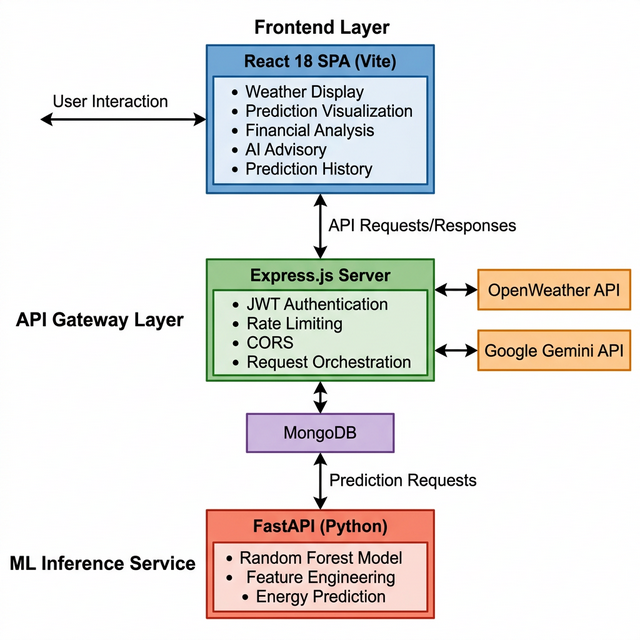
\includegraphics[width=\columnwidth]{fig_architecture.png}
\caption{Three-tier microservice architecture of SolarPredict. The React frontend communicates with the Express.js API gateway, which orchestrates the ML inference service, Generative AI planning service, external weather APIs, and persistent MongoDB storage.}
\label{fig:arch}
\end{figure}

\subsection{Data Flow Pipeline}

The end-to-end prediction and planning pipeline operates through the following sequence:

\begin{enumerate}
\item The user inputs their city name and solar panel capacity (kW) through the React frontend interface.
\item The Express.js backend invokes the OpenWeather API to retrieve current weather conditions and a 5-day forecast for the specified location.
\item Weather parameters (temperature, humidity, cloud cover percentage, wind speed) along with panel capacity and geographic latitude are forwarded to the FastAPI ML service.
\item The ML service constructs 96 feature vectors (one per 15-minute interval over 24 hours) for each forecast day, incorporating cyclical time encodings and physics-informed solar geometry calculations.
\item The Random Forest model predicts normalized power output for each interval, which is subsequently scaled by panel capacity and a system loss factor of 82\% to produce energy estimates in kWh.
\item The API gateway augments predictions with financial analysis (costs, subsidies, ROI), then forwards the complete context to the Google Gemini Generative AI service for natural language summary generation and planning recommendations.
\item The consolidated response---comprising predictions, financial analysis, AI advisory, and appliance scheduling recommendations---is transmitted to the frontend for interactive visualization.
\end{enumerate}

\subsection{Technology Stack}

Table~\ref{tab:tech} summarizes the technology stack employed across the system layers.

\begin{table}[H]
\caption{Technology Stack Summary}
\begin{center}
\small
\begin{tabular}{|l|l|}
\hline
\textbf{Layer} & \textbf{Technologies} \\
\hline
Frontend & React 18, Vite, Recharts, Axios \\
\hline
Backend API & Node.js, Express.js, Mongoose, JWT \\
\hline
ML Service & Python 3.x, FastAPI, scikit-learn, joblib \\
\hline
Gen AI Planning & Google Gemini 2.0 Flash LLM \\
\hline
Database & MongoDB (Atlas) \\
\hline
External APIs & OpenWeather API v2.5 \\
\hline
\end{tabular}
\label{tab:tech}
\end{center}
\end{table}

\section{Machine Learning Model}

\subsection{Dataset Description}

The prediction model is trained on real-world operational data obtained from the ``Solar Power Generation Data'' dataset published on Kaggle \cite{b12}. The dataset comprises generation and weather sensor measurements from two solar power plants, organized into four CSV files: Plant\_1\_Generation\_Data.csv, Plant\_1\_Weather\_Sensor\_Data.csv, Plant\_2\_Generation\_Data.csv, and Plant\_2\_Weather\_Sensor\_Data.csv. The generation data contains timestamped AC and DC power output readings per inverter, while the weather data includes ambient temperature, module temperature, and solar irradiation measurements. The combined dataset encompasses 136,476 records across 44 unique inverters spanning a temporal range from May to June 2020.

\subsection{Feature Engineering}

Nine features are systematically engineered from the raw data to capture the principal physical and temporal factors governing solar energy generation:

\begin{enumerate}
\item \textbf{Irradiation}: Direct measurement of solar irradiance (kW/m\textsuperscript{2}) from on-site weather sensors, serving as the primary surrogate for incident solar energy.
\item \textbf{Ambient Temperature}: Measured atmospheric air temperature (\textdegree C) at the plant site, influencing photovoltaic cell efficiency through temperature-dependent semiconductor behavior.
\item \textbf{Humidity}: Synthesized proxy variable inversely correlated with temperature and irradiation, representing atmospheric moisture content that attenuates solar radiation through absorption and scattering.
\item \textbf{Cloud Cover}: Derived as the inverse of measured irradiation relative to the 99th percentile clear-sky irradiance reference, capturing the fractional sky obscuration.
\item \textbf{Wind Speed}: Generated proxy variable with temperature-correlated convective variation and stochastic Gaussian noise, modeling the cooling effect on panel surface temperature.
\item \textbf{Hour Sine and Cosine}: Cyclical encoding of the hour of day using $\sin(2\pi h/24)$ and $\cos(2\pi h/24)$, eliminating the artificial discontinuity at midnight inherent in raw hour representations.
\item \textbf{Day-of-Year Sine and Cosine}: Cyclical encoding of the ordinal day using $\sin(2\pi d/365)$ and $\cos(2\pi d/365)$, capturing seasonal variation in solar declination and day length.
\end{enumerate}

The prediction target is the normalized AC power output, computed as:

\begin{equation}
y_{\text{norm}} = \frac{P_{\text{AC}}}{P_{99}^{(i)}}
\label{eq:norm}
\end{equation}

where $P_{\text{AC}}$ denotes the measured AC power output and $P_{99}^{(i)}$ represents the 99th percentile AC power for inverter $i$, calculated from the training partition. This per-inverter normalization strategy accommodates heterogeneous inverter capacities and efficiencies across the two plant installations.

\subsection{Model Training and Hyperparameters}

A Random Forest Regressor is trained with the hyperparameter configuration detailed in Table~\ref{tab:hyperparams}.

\begin{table}[H]
\caption{Random Forest Hyperparameter Configuration}
\begin{center}
\small
\begin{tabular}{|l|c|}
\hline
\textbf{Hyperparameter} & \textbf{Value} \\
\hline
Number of estimators (trees) & 200 \\
\hline
Maximum tree depth & 20 \\
\hline
Minimum samples per leaf & 2 \\
\hline
Random state seed & 42 \\
\hline
Parallel jobs & $-1$ (all cores) \\
\hline
\end{tabular}
\label{tab:hyperparams}
\end{center}
\end{table}

The dataset is partitioned temporally using an 80/20 ratio with a split timestamp of 2020-06-11T12:30:00 UTC, ensuring that the test set comprises exclusively future data unseen during model training. This temporal partitioning strategy is deliberately chosen over random splitting to faithfully simulate real-world deployment conditions where the model must predict future energy output based on patterns learned from historical observations.

\subsection{Inference Pipeline}

During inference, the system constructs feature vectors for each 15-minute interval spanning a full 24-hour day. Solar irradiance is estimated using a physics-informed model incorporating:

\begin{itemize}
\item Solar declination angle computed from the day of year
\item Hour angle for sub-daily solar position variation
\item Latitude-dependent zenith angle calculation
\item Cloud cover attenuation factor: $f_c = \max(0.08, 1 - 0.75 \cdot c^{1.2})$
\item Humidity scattering factor: $f_h = \max(0.75, 1 - 0.20 \cdot h)$
\end{itemize}

where $c$ and $h$ are the normalized cloud cover and humidity values, respectively. The model's normalized power predictions are then converted to absolute energy estimates:

\begin{equation}
E_{\text{daily}} = \sum_{t=1}^{96} \hat{y}_t \cdot C_p \cdot \eta_s \cdot \Delta t
\label{eq:energy}
\end{equation}

where $\hat{y}_t$ is the predicted normalized power at interval $t$, $C_p$ is the panel capacity (kW), $\eta_s = 0.82$ is the composite system loss factor accounting for inverter conversion losses, wiring resistance, and surface soiling, and $\Delta t = 0.25$~hours.

Panel efficiency is further modulated by temperature effects according to:

\begin{equation}
\eta_T = \eta_{\text{base}} \cdot \left(1 + k_T \cdot (T_{\text{cell}} - T_{\text{STC}})\right)
\label{eq:temp}
\end{equation}

where $k_T = -0.004~\text{per}~^\circ\text{C}$ is the temperature coefficient for crystalline silicon cells, $T_{\text{cell}} = T_{\text{ambient}} + 25^\circ\text{C}$ is the estimated cell temperature, and $T_{\text{STC}} = 25^\circ\text{C}$ is the standard test condition reference temperature.

\section{Generative AI Planning System and Decision Support Features}

\subsection{Generative AI-Powered Planning and Advisory}

A distinguishing feature of SolarPredict is its Generative AI-based planning system, which leverages the Google Gemini 2.0 Flash large language model to transform quantitative ML predictions into qualitative, actionable planning guidance. The AI planning module operates in two complementary modes:

\begin{enumerate}
\item \textbf{Automated Summary and Planning Mode}: Upon generation of prediction results, the system automatically constructs a structured prompt containing the user's location, weather data, energy predictions, financial analysis, and subsidy information. The Gemini LLM processes this context to generate a concise, non-technical narrative summarizing the user's solar potential, estimated savings, environmental impact, and a practical implementation recommendation. This mode enables users without technical expertise to immediately understand the implications of the prediction output.

\item \textbf{Interactive Q\&A Planning Mode}: Users can submit free-form natural language questions regarding any aspect of their solar investment---including savings projections, subsidy eligibility, ROI timelines, maintenance schedules, panel selection, and energy optimization strategies. The system constructs a context-enriched prompt incorporating the user's prediction data and financial analysis, enabling the LLM to provide personalized, data-grounded responses rather than generic information.
\end{enumerate}

A robust fallback mechanism utilizing rule-based response templates ensures uninterrupted service continuity when the Generative AI API encounters rate limiting, network timeouts, or temporary unavailability.

\subsection{Financial Analysis Engine}

The system incorporates a comprehensive financial analysis module tailored specifically to the Indian residential solar market. Installation costs are modeled as a function of system capacity using tiered per-kW rates ranging from INR~42,000 for systems exceeding 10~kW to INR~65,000 for 1~kW systems, reflecting current 2024--2025 market pricing. Government subsidies under the PM Surya Ghar scheme are calculated according to:

\begin{equation}
S = \begin{cases}
30{,}000 \cdot C & \text{if } C \leq 2~\text{kW} \\
60{,}000 + 18{,}000 \cdot (C - 2) & \text{if } 2 < C \leq 3~\text{kW} \\
78{,}000 & \text{if } C > 3~\text{kW}
\end{cases}
\label{eq:subsidy}
\end{equation}

where $S$ denotes the subsidy amount in INR and $C$ represents the system capacity in kW.

The ROI computation incorporates the following parameters:
\begin{itemize}
\item State-specific electricity tariff rates for 15 Indian states
\item 0.5\% annual panel degradation factor
\item 5\% annual electricity rate escalation assumption
\item INR~2,000 annual maintenance cost provision
\item 25-year cumulative net savings projection
\item CO\textsubscript{2} emission offset at 0.82~kg per kWh (Indian grid emission factor)
\end{itemize}

Users can optionally input their current monthly electricity bill for a personalized bill comparison analysis showing the estimated post-solar adoption bill, monthly savings, and payback acceleration.

\subsection{Smart Appliance Scheduling}

The planning system generates intelligent appliance usage schedules based on predicted peak solar generation windows. High-power appliances (washing machine, water heater, air conditioner) are recommended for operation during peak solar hours (typically 10:00~AM--3:00~PM), thereby maximizing self-consumption of solar energy. Forecast-aware alerts proactively notify users to shift energy-intensive loads when the succeeding day's predicted output deviates by more than 20\% from the current day's generation.

\subsection{User Authentication and Prediction History}

JWT-based authentication enables registered users to persist prediction results to MongoDB and access their complete prediction history. This longitudinal tracking capability facilitates seasonal performance comparison, trend analysis, and validation of prediction accuracy against observed generation data over time.

\section{Experimental Results and Analysis}

\subsection{Model Performance Evaluation}

The trained Random Forest model is evaluated on the temporally partitioned test set comprising 27,280 records. Table~\ref{tab:metrics} presents the comprehensive performance metrics.

\begin{table}[H]
\caption{Random Forest Model Performance Metrics}
\begin{center}
\small
\begin{tabular}{|l|c|}
\hline
\textbf{Metric} & \textbf{Value} \\
\hline
Normalized R\textsuperscript{2} Score & 0.8534 \\
\hline
Normalized MAE & 0.0319 \\
\hline
Absolute R\textsuperscript{2} Score & 0.8578 \\
\hline
Absolute MAE (Watts) & 39.28 \\
\hline
Training Samples & 109,196 \\
\hline
Test Samples & 27,280 \\
\hline
Number of Inverters & 44 \\
\hline
\end{tabular}
\label{tab:metrics}
\end{center}
\end{table}

The normalized R\textsuperscript{2} of 0.8534 exceeds the predefined baseline threshold of 0.82, indicating that the model explains approximately 85\% of the variance in normalized power output. The normalized MAE of 0.0319 is substantially below the acceptable threshold of 0.05, confirming tight prediction accuracy. These metrics collectively validate the model's capacity to generalize across temporal boundaries and heterogeneous inverter configurations.

The absolute metrics further corroborate model quality: an R\textsuperscript{2} of 0.8578 on raw wattage predictions and an MAE of 39.28~W demonstrate that prediction errors remain small relative to typical inverter output ranges spanning 0--2,000~W.

\subsection{Baseline Model Comparison}

To justify the selection of Random Forest as the prediction model, we compare its performance against two baseline models---Linear Regression and a single Decision Tree---trained and evaluated on the identical temporal split. Table~\ref{tab:baseline} presents the comparative results.

\begin{table}[H]
\caption{Comparison of ML Models on Normalized Test Set}
\begin{center}
\small
\begin{tabular}{|l|c|c|c|}
\hline
\textbf{Model} & \textbf{R\textsuperscript{2}} & \textbf{MAE} & \textbf{Train Time} \\
\hline
Linear Regression & 0.8336 & 0.0504 & 0.04~s \\
\hline
Decision Tree & 0.8134 & 0.0344 & 0.65~s \\
\hline
\textbf{Random Forest} & \textbf{0.8531} & \textbf{0.0319} & 74.17~s \\
\hline
\end{tabular}
\label{tab:baseline}
\end{center}
\end{table}

Random Forest achieves the highest R\textsuperscript{2} (0.8531) and the lowest MAE (0.0319) among all evaluated models. Linear Regression attains a comparable R\textsuperscript{2} of 0.8336 but exhibits a substantially higher MAE (0.0504), exceeding the acceptable threshold of 0.05 and indicating poor prediction tightness for individual intervals. The single Decision Tree overfits to localized patterns, yielding the lowest R\textsuperscript{2} (0.8134). The ensemble averaging in Random Forest effectively mitigates this overfitting while retaining the Decision Tree's capacity for capturing nonlinear feature interactions, justifying the increased training time.

\subsection{Feature Importance Analysis}

Fig.~\ref{fig:feat} and Table~\ref{tab:importance} present the feature importance scores derived from the trained Random Forest model using the mean decrease in impurity criterion.

\begin{table}[H]
\caption{Feature Importance Scores from Random Forest Model}
\begin{center}
\small
\begin{tabular}{|l|c|}
\hline
\textbf{Feature} & \textbf{Importance} \\
\hline
Irradiation & 0.8312 \\
\hline
Wind Speed & 0.0636 \\
\hline
Cloud Cover & 0.0397 \\
\hline
Ambient Temperature & 0.0196 \\
\hline
Humidity & 0.0122 \\
\hline
Day-of-Year Sine & 0.0100 \\
\hline
Day-of-Year Cosine & 0.0100 \\
\hline
Hour Sine & 0.0088 \\
\hline
Hour Cosine & 0.0049 \\
\hline
\end{tabular}
\label{tab:importance}
\end{center}
\end{table}

Irradiation dominates with an importance score of 0.8312, unequivocally confirming its role as the primary determinant of solar power output. This finding aligns with established photovoltaic theory, as the photocurrent generated by PV cells is directly proportional to incident irradiance. The secondary features---wind speed (0.0636), cloud cover (0.0397), and ambient temperature (0.0196)---collectively capture the atmospheric conditions that modulate panel performance through cooling effects, light attenuation, and temperature-dependent efficiency variations. The cyclical time features contribute modestly (combined 0.0337), as their temporal information is substantially encoded within the irradiation measurements themselves.

\begin{figure}[H]
\centering
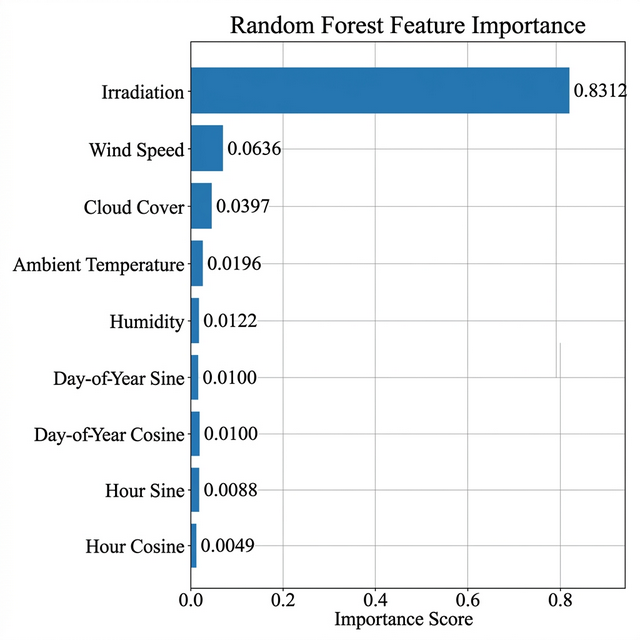
\includegraphics[width=\columnwidth]{fig_feature_importance.png}
\caption{Feature importance scores from the Random Forest model demonstrating the dominant contribution of irradiation (0.8312) in predicting solar power output, followed by secondary meteorological features.}
\label{fig:feat}
\end{figure}

\subsection{System Performance Analysis}

The complete prediction and planning pipeline---from weather API invocation through ML inference to Generative AI advisory generation---executes within 3--5 seconds under typical network conditions. The FastAPI ML inference service processes a single-day prediction request (96 feature vectors) in under 100~milliseconds on commodity hardware. The Express.js API gateway sustains 100 concurrent requests per 15-minute window with rate limiting, ensuring equitable resource allocation across concurrent users. The Generative AI planning component adds approximately 1--2 seconds of latency for LLM-based summary and recommendation generation, which is acceptable for the interactive use case.

\subsection{Web Application Output}

Fig.~\ref{fig:output1} and Fig.~\ref{fig:output2} illustrate the SolarPredict web application interface, demonstrating the prediction dashboard and the AI-powered planning advisory output respectively.

\begin{figure}[H]
\centering
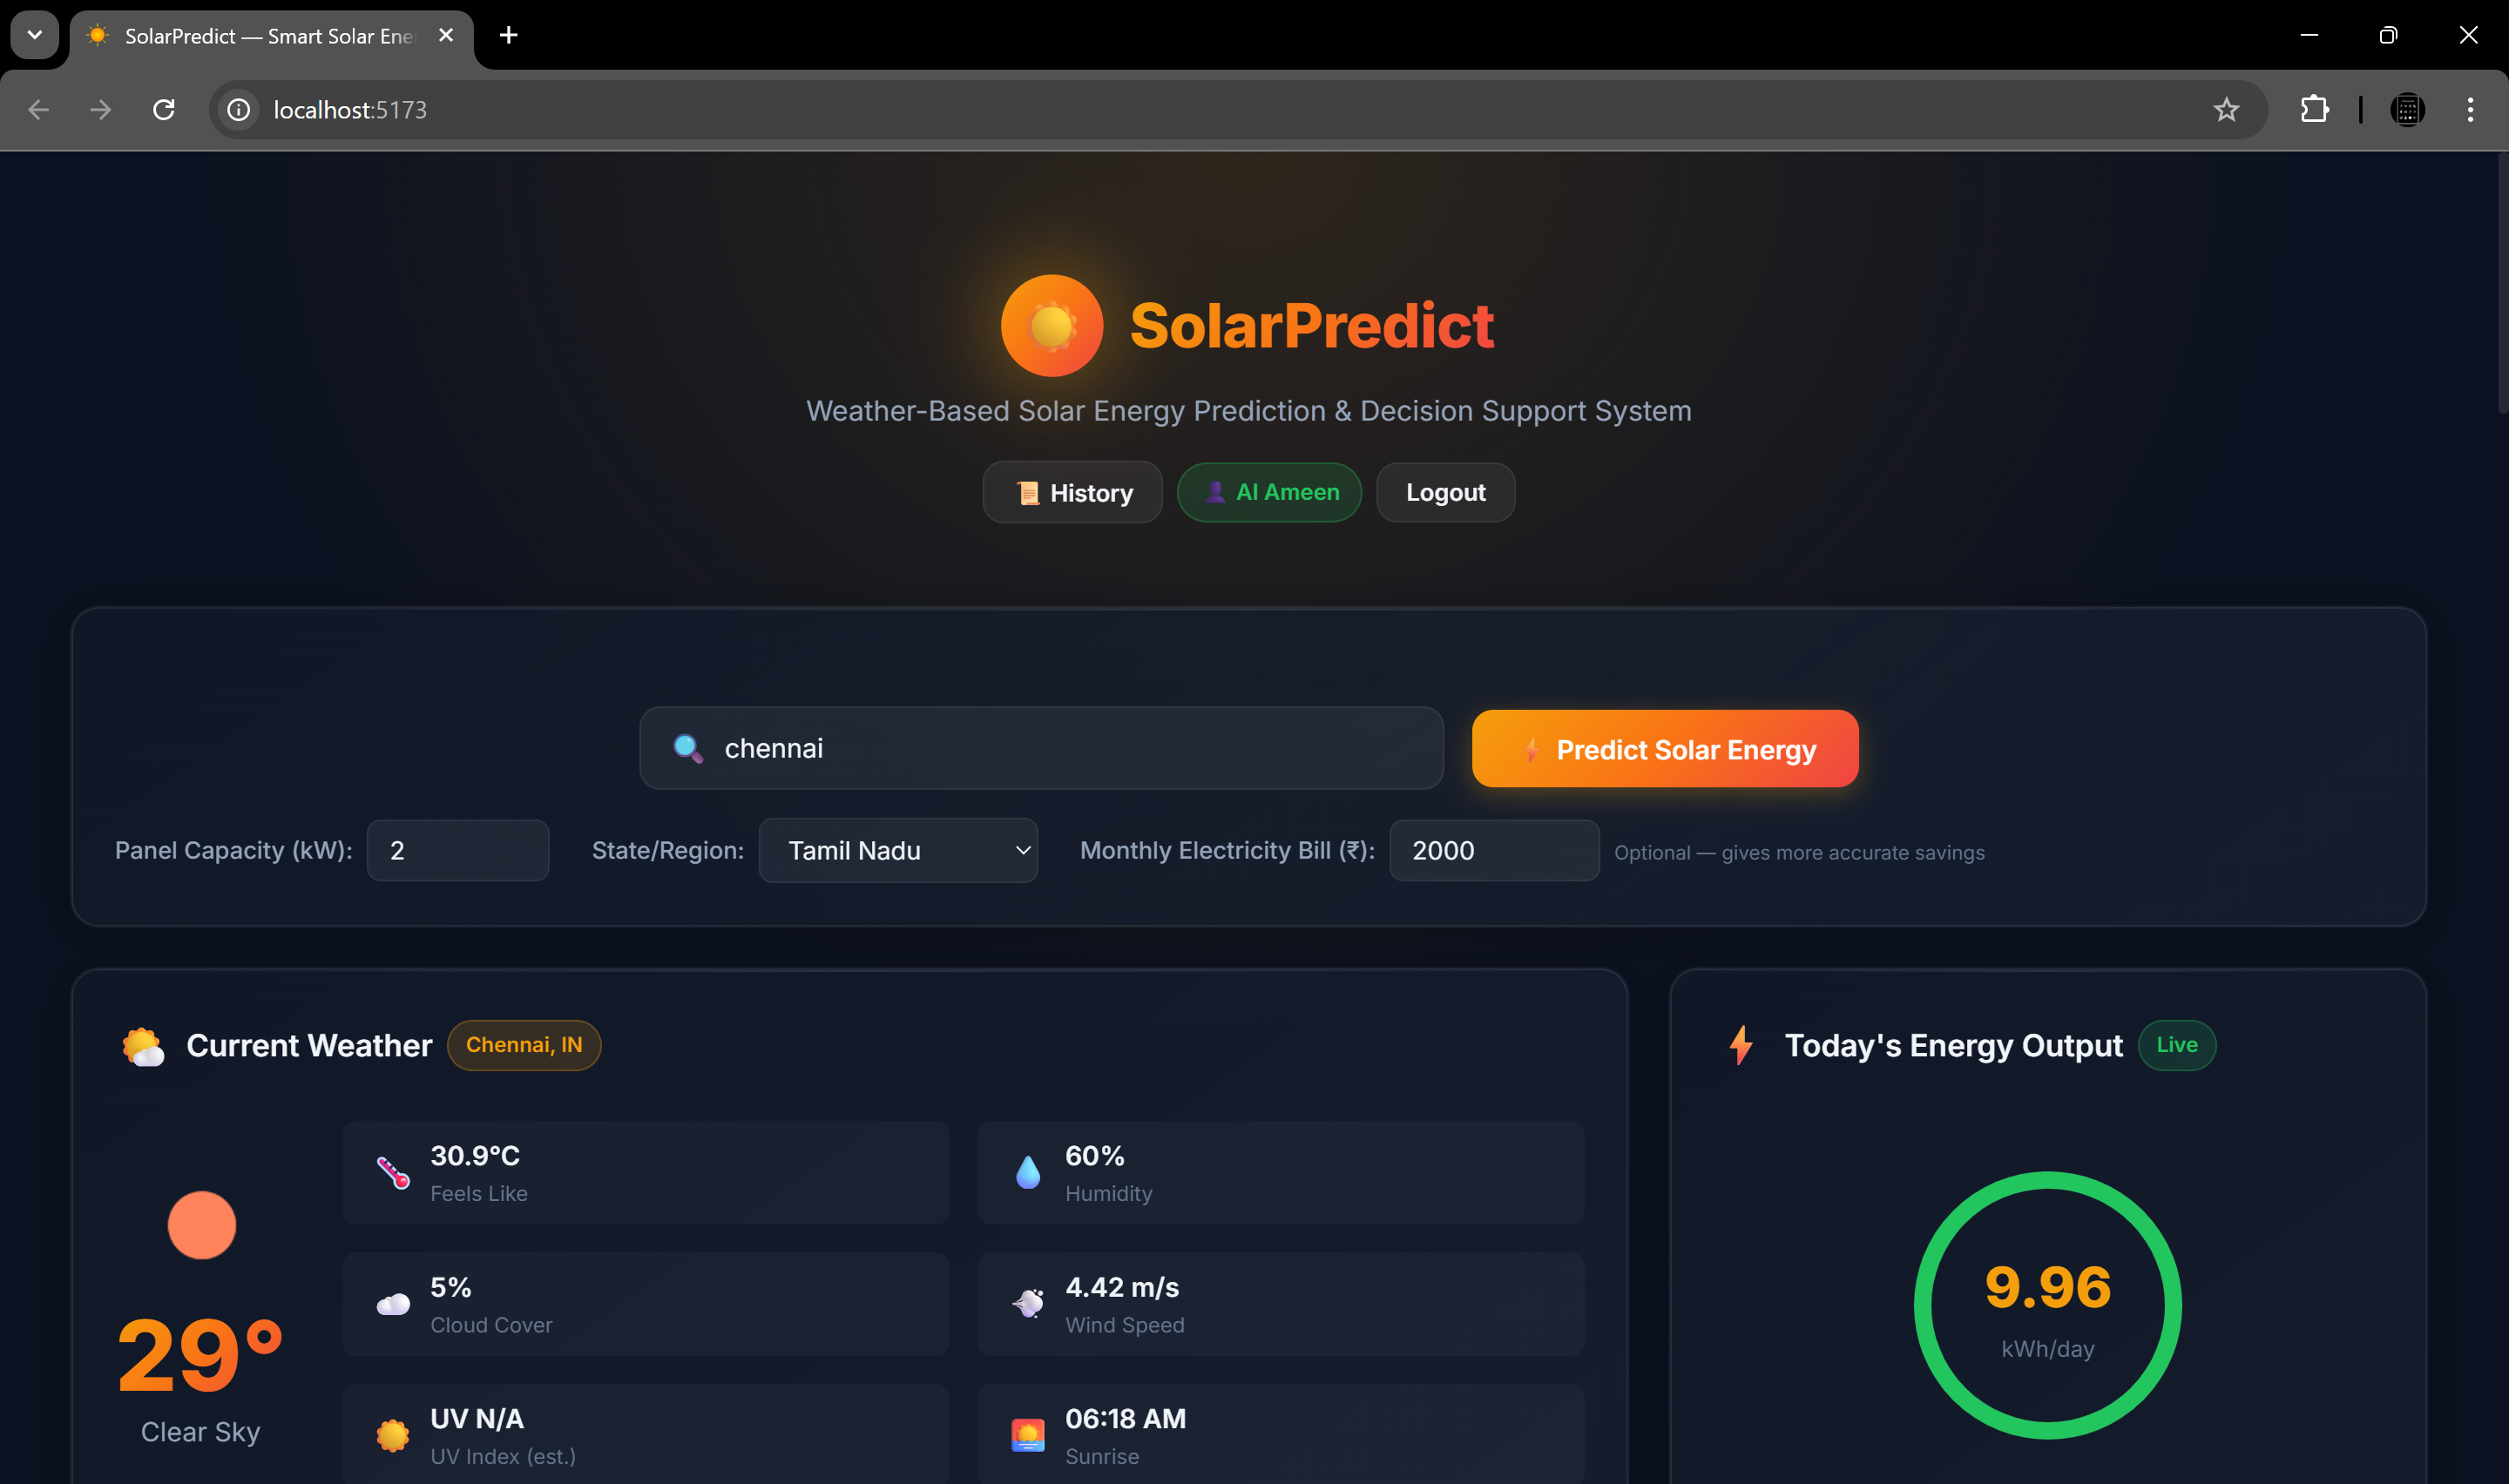
\includegraphics[width=\columnwidth]{fig_output1.png}
\caption{SolarPredict web application --- prediction dashboard showing real-time weather data, energy forecast visualization, and current energy output summary for a user in Chennai.}
\label{fig:output1}
\end{figure}

\begin{figure}[H]
\centering
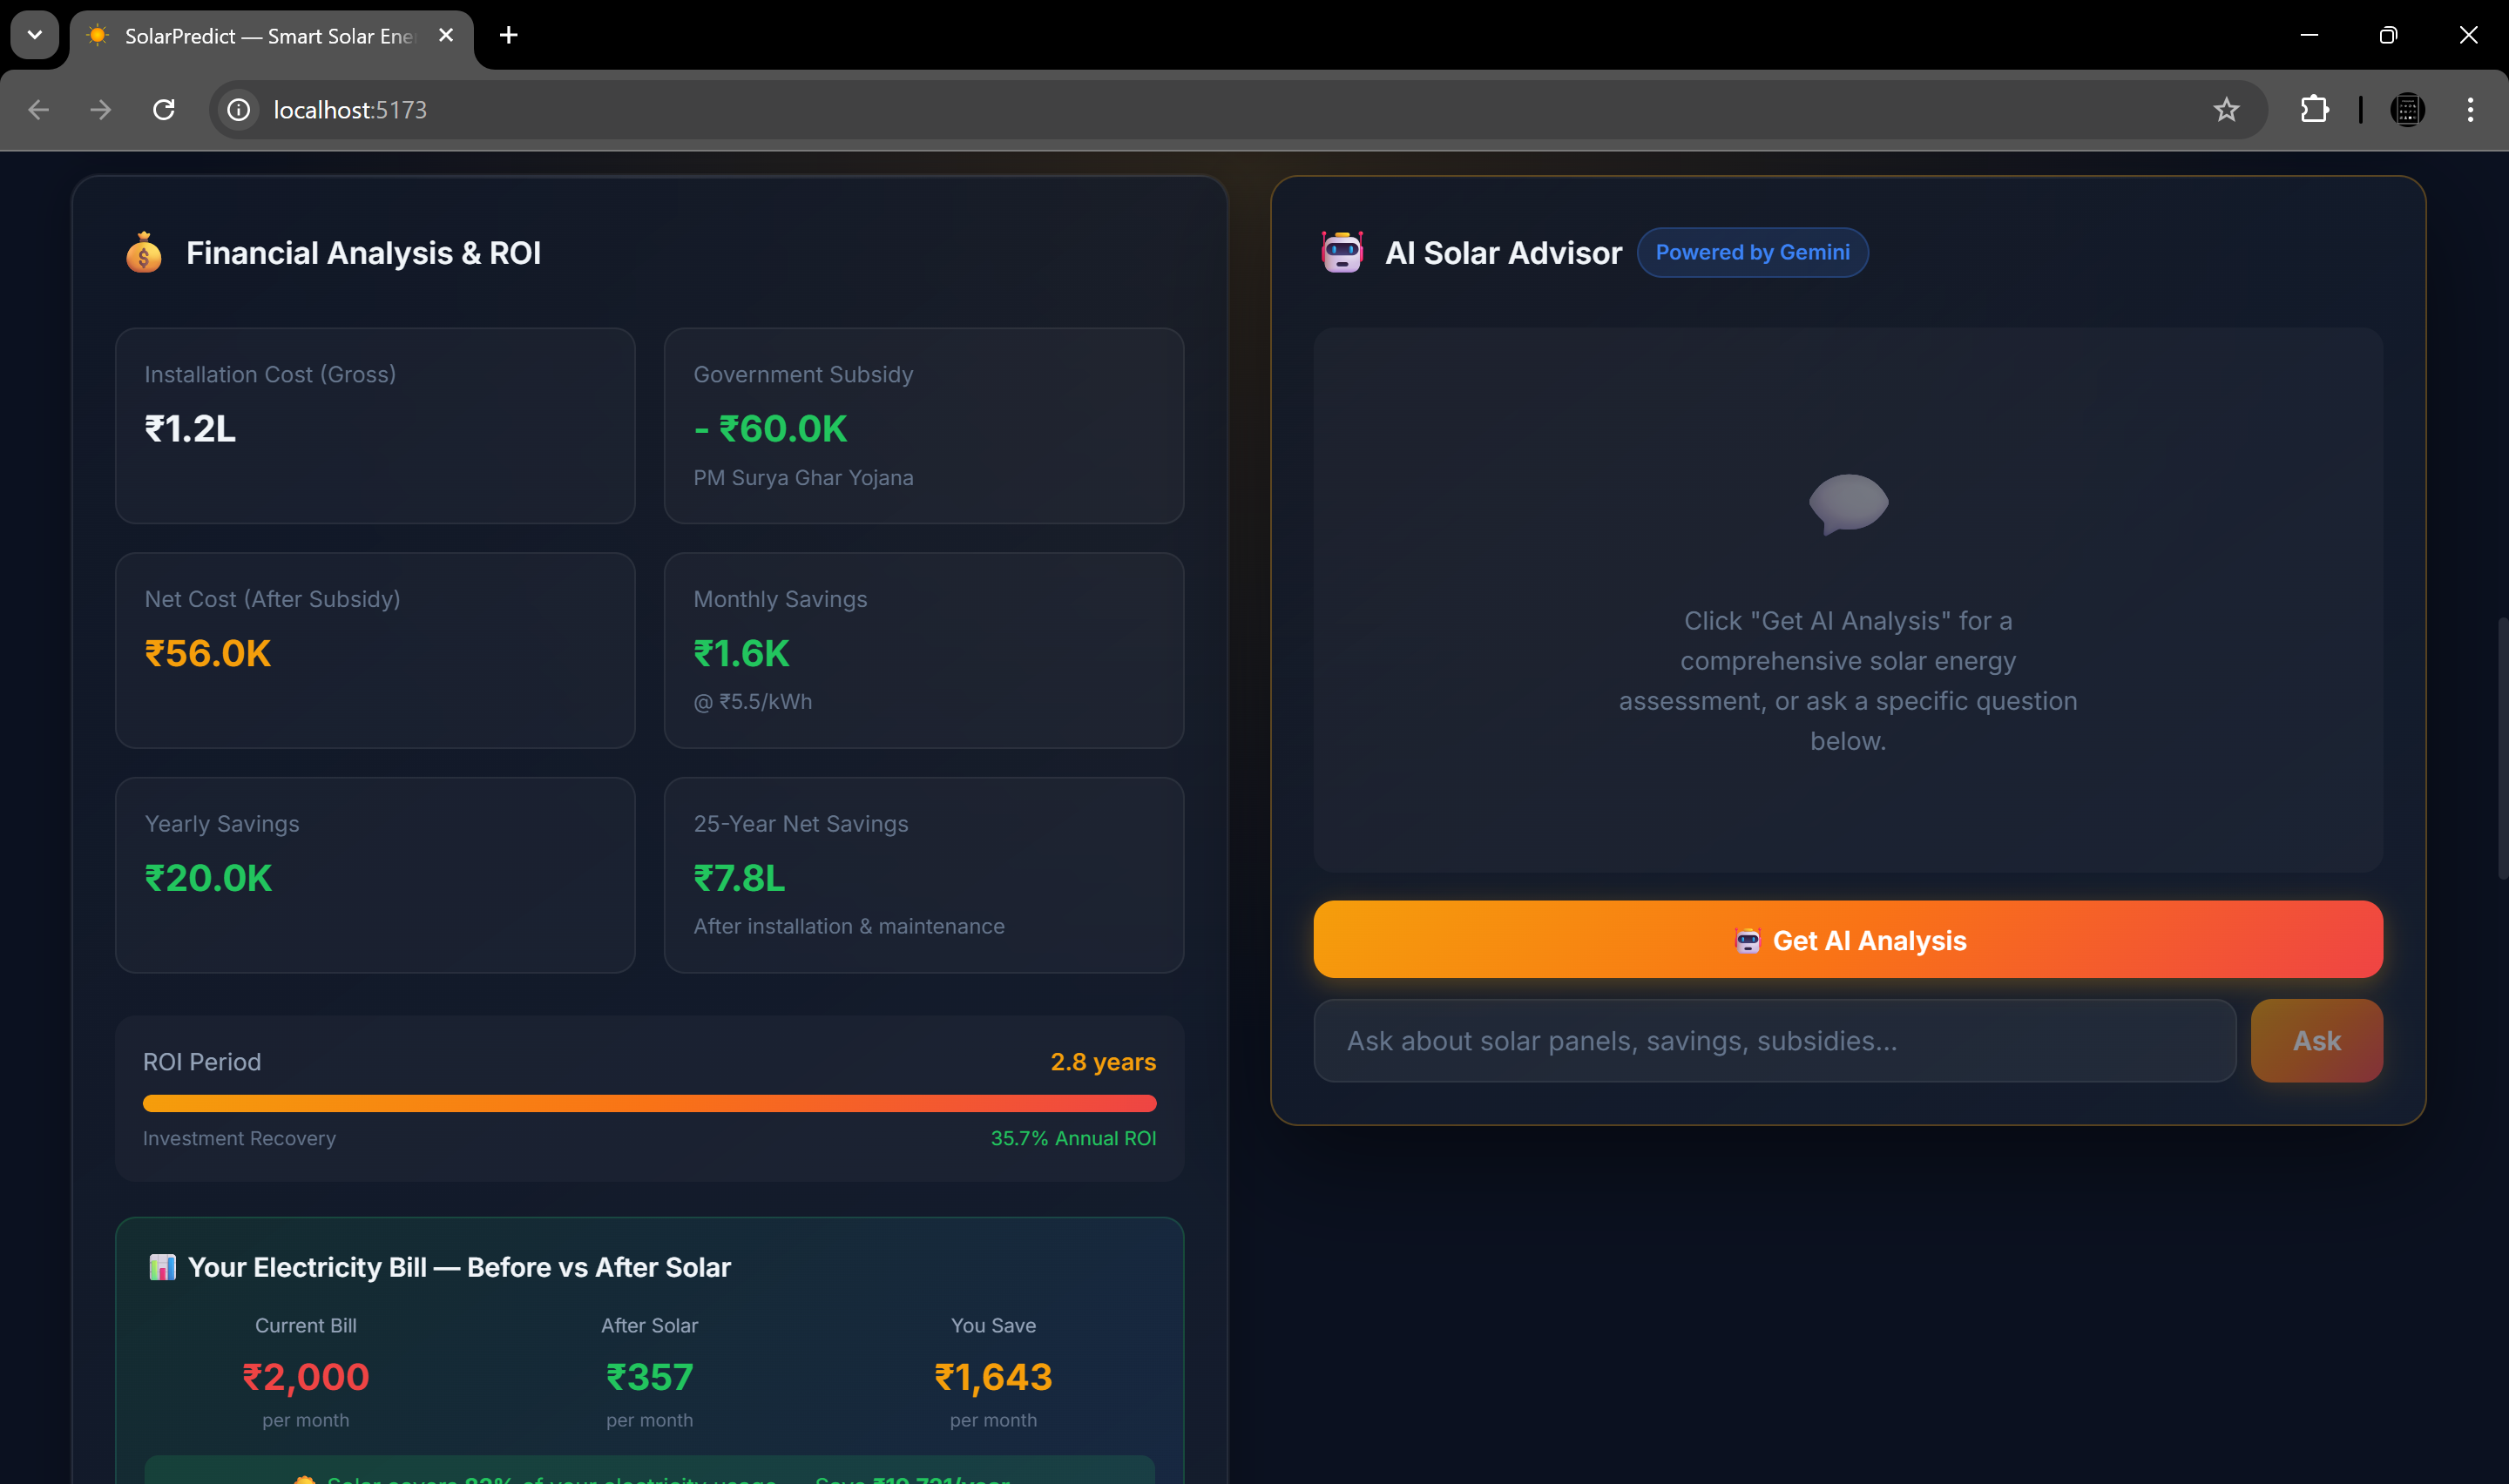
\includegraphics[width=\columnwidth]{fig_output2.png}
\caption{SolarPredict web application --- financial analysis and ROI dashboard with the Generative AI-powered Solar Advisor interface for interactive planning and Q\&A.}
\label{fig:output2}
\end{figure}

\subsection{Comparison with Existing Approaches}

Table~\ref{tab:comparison} provides a qualitative comparison of SolarPredict with existing solar estimation tools, highlighting the unique combination of ML-based prediction, Generative AI planning, and India-specific financial modeling.

\begin{table}[H]
\caption{Comparison with Existing Solar Estimation Tools}
\begin{center}
\footnotesize
\begin{tabular}{|l|c|c|c|}
\hline
\textbf{Feature} & \textbf{SolarPredict} & \textbf{PVWatts} & \textbf{Sunroof} \\
\hline
ML Prediction & \checkmark & $\times$ & $\times$ \\
\hline
Gen AI Planning & \checkmark & $\times$ & $\times$ \\
\hline
Real-time Weather & \checkmark & $\times$ & $\times$ \\
\hline
India Subsidies & \checkmark & $\times$ & $\times$ \\
\hline
Smart Scheduling & \checkmark & $\times$ & $\times$ \\
\hline
Bill Comparison & \checkmark & Partial & $\times$ \\
\hline
User History & \checkmark & $\times$ & $\times$ \\
\hline
\end{tabular}
\label{tab:comparison}
\end{center}
\end{table}

\section{Conclusion and Future Work}

This paper presented SolarPredict, a comprehensive weather-based solar energy prediction and Generative AI-powered planning system designed specifically for Indian residential consumers. The system integrates a Random Forest regression model achieving an R\textsuperscript{2} of 0.853 with real-time weather data, detailed financial analysis including government subsidy calculations, and a Generative AI planning module powered by Google Gemini for personalized advisory services and smart energy management recommendations. The three-tier microservice architecture ensures modularity, independent scalability, and maintainability of each system component.

The principal contributions of this work include: (1)~a feature engineering pipeline that synthesizes real weather measurements with derived atmospheric parameters and cyclical time encodings; (2)~a per-inverter P99 normalization strategy enabling model generalization across heterogeneous inverter configurations; (3)~integration of comprehensive financial modeling specific to the Indian market encompassing PM Surya Ghar subsidy calculations and state-wise tariff structures; and (4)~a Generative AI-augmented planning system that translates technical ML predictions into actionable natural language recommendations for non-technical residential consumers.

Several limitations of the current work are acknowledged. First, three of the nine input features---humidity, cloud cover, and wind speed---are synthesized proxy variables derived from temperature and irradiation measurements rather than direct sensor readings; incorporating real meteorological station data for these parameters would improve prediction fidelity. Second, the training dataset spans a limited temporal window of approximately two months (May--June 2020), which constrains the model's ability to capture full seasonal variation in solar generation patterns. The cyclical day-of-year features provide partial seasonal extrapolation capability, but validation against data spanning a complete annual cycle remains necessary.

Future research directions include: (a)~evaluating additional ML architectures including Gradient Boosting Machines and Long Short-Term Memory (LSTM) networks for ensemble prediction; (b)~incorporating satellite-derived irradiance data and real meteorological measurements for broader geographic coverage and improved feature quality; (c)~adding battery storage optimization and net metering simulation capabilities; (d)~developing a mobile application for wider accessibility; (e)~implementing multi-turn conversational planning with memory-augmented Generative AI; and (f)~conducting field validation against actual metered generation data from rooftop installations across diverse Indian climatic zones.

\section*{Acknowledgment}

The authors gratefully acknowledge the use of the Solar Power Generation Dataset made publicly available on Kaggle \cite{b12}. The OpenWeather API was used for real-time meteorological data, and the Google Gemini API was employed for Generative AI-based planning and advisory services. The authors also thank the Department of Information Technology, Dhanalakshmi Srinivasan College of Engineering and Technology, for institutional support.

\begin{thebibliography}{00}
\bibitem{b1} Ministry of New and Renewable Energy, Government of India, ``India's updated first Nationally Determined Contribution under Paris Agreement,'' 2023. [Online]. Available: https://mnre.gov.in/

\bibitem{b2} Press Information Bureau, ``PM Surya Ghar: Muft Bijli Yojana - Rooftop Solar Scheme,'' Government of India, 2024. [Online]. Available: https://pmsuryaghar.gov.in/

\bibitem{b3} R. Ahmed, V. Sreeram, Y. Mishra, and M. D. Arif, ``A review and evaluation of the state-of-the-art in PV solar power forecasting: techniques and optimization,'' \textit{Renewable and Sustainable Energy Reviews}, vol. 124, p. 109792, 2020.

\bibitem{b4} A. Mellit and A. M. Pavan, ``A 24-h forecast of solar irradiance using artificial neural network: application for performance prediction of a grid-connected PV plant at Trieste, Italy,'' \textit{Solar Energy}, vol. 84, no. 5, pp. 807--821, 2010.

\bibitem{b5} M. Abuella and B. Chowdhury, ``Forecasting of solar power ramp events: a post-processing approach,'' \textit{Renewable Energy}, vol. 133, pp. 1380--1392, 2019.

\bibitem{b6} H. C. Hottel, ``A simple model for estimating the transmittance of direct solar radiation through clear atmospheres,'' \textit{Solar Energy}, vol. 18, no. 2, pp. 129--134, 1976.

\bibitem{b7} C. Voyant, G. Notton, S. Kalogirou, M.-L. Nivet, C. Paoli, F. Motte, and A. Fouilloy, ``Machine learning methods for solar radiation forecasting: a review,'' \textit{Renewable Energy}, vol. 105, pp. 569--582, 2017.

\bibitem{b8} L. Breiman, ``Random forests,'' \textit{Machine Learning}, vol. 45, no. 1, pp. 5--32, 2001.

\bibitem{b9} Google, ``Project Sunroof -- Solar savings estimator,'' 2023. [Online]. Available: https://sunroof.withgoogle.com/

\bibitem{b10} National Renewable Energy Laboratory, ``PVWatts Calculator,'' 2024. [Online]. Available: https://pvwatts.nrel.gov/

\bibitem{b11} J. Chen, X. Liang, and Z. Li, ``Large language models for energy systems: a survey,'' \textit{arXiv preprint arXiv:2312.15719}, 2023.

\bibitem{b12} Afroz, ``Solar Power Generation Data,'' Kaggle, 2020. [Online]. Available: https://www.kaggle.com/datasets/anikannal/solar-power-generation-data

\bibitem{b13} M. Abdel-Nasser and K. Mahmoud, ``Accurate photovoltaic power forecasting models using deep LSTM-RNN,'' \textit{Neural Computing and Applications}, vol. 31, no. 7, pp. 2727--2740, 2019.

\bibitem{b14} J. Antonanzas, N. Osorio, R. Escobar, R. Urraca, F. J. Martinez-de-Pison, and F. Antonanzas-Torres, ``Review of photovoltaic power forecasting,'' \textit{Solar Energy}, vol. 136, pp. 78--111, 2016.

\bibitem{b15} V. Kushwaha and N. M. Pindoriya, ``A SARIMA-RVFL hybrid model assisted by wavelet decomposition for very short-term solar PV power generation forecast,'' \textit{Renewable Energy}, vol. 140, pp. 124--139, 2019.

\bibitem{b16} S. Sobri, S. Koohi-Kamali, and N. A. Rahim, ``Solar photovoltaic generation forecasting methods: a review,'' \textit{Energy Conversion and Management}, vol. 156, pp. 459--497, 2018.

\bibitem{b17} P. Kumari and D. Toshniwal, ``Deep learning models for solar irradiance forecasting: a comprehensive review,'' \textit{Journal of Cleaner Production}, vol. 318, p. 128566, 2021.

\bibitem{b18} H. T. C. Pedro and C. F. M. Coimbra, ``Assessment of forecasting techniques for solar power production with no exogenous inputs,'' \textit{Solar Energy}, vol. 86, no. 7, pp. 2017--2028, 2012.

\bibitem{b19} M. Q. Raza, M. Nadarajah, and C. Ekanayake, ``On recent advances in PV output power forecast,'' \textit{Solar Energy}, vol. 136, pp. 125--144, 2016.

\bibitem{b20} A. Srivastava and D. K. Seshadri, ``An analysis of rooftop solar PV potential in Indian states using geographic information system,'' \textit{Current Science}, vol. 121, no. 8, pp. 1052--1060, 2021.
\end{thebibliography}

\end{document}
